\textbf{Цель работы:} исследовать свойства постоянных неодимовых магнитов;
измерить с их помощью горизонтальную и вертикальную составляющие
индукции магнитного поля Земли и магнитное наклонение.\\\indent
\textbf{Оборудование:} неодимовые магниты; тонкая нить для изготов­
ления крутильного маятника; медная проволока; электронные весы; секун­
домер; измеритель магнитной индукции; штангенциркуль; брусок, линейка
и штатив из немагнитных материалов; набор гирь и разновесов.
\section*{Теоретические сведения}
Магнитное поле точечного диполя определяется как:
\begin{equation}
    \bar{B}_{\text{дип}}(\bar{r}) = \frac{\mu_0}{4\pi}\left (\frac{3(\bar{\mathfrak{m}}\cdot \bar{r})\bar{r}}{r^5} - \frac{\bar{\mathfrak{m}}}{r^3}\right )
\end{equation}
где $m$ - магнитный момент.\\ 
\indent Во внешнем магнитном поле с индукцией $\bar{B}$ на точечный магнитный
диполь $\bar{\mathfrak{m}}$ действует механический момент сил:
\begin{equation}
    \bar{M} = [\bar{\mathfrak{m}} \times \bar{B}]
\end{equation}
Потенциальная работа при этом:
\begin{equation}
    W = - (\bar{\mathfrak{m}} \cdot \bar{B})
\end{equation}
В неоднородном внешнем поле кроме момента сил на диполь действует еще сила:
\begin{equation}
    \bar{F} = -\nabla W = (\bar{\mathfrak{m}}\cdot \nabla)\bar{B}
\end{equation}
Тогда по этим формулам рассчитаем силу взаимодействия магнитов с мометами $\bar{\mathfrak{m_1}}$ и $\bar{\mathfrak{m_2}}$ направленные вдоль соединяющей их прямой $\bar{r}$:
\begin{equation}
    F_{12} = \mathfrak{m_1}\frac{\partial B_2}{\partial r} = \mathfrak{m_1} \frac{\partial{(2 \mathfrak{m_2}/r^3})}{\partial r} = -\frac{6\mathfrak{m_1} \mathfrak{m_2}}{r^4}
\end{equation}
Если $\bar{m_{12}} \perp \bar{r}$:
\begin{equation}
    F_{12} = \frac{3\mathfrak{m_1 m_2}}{r^4}
\end{equation}
Еще одной характеристихой материала магнита является намагниченность $\mathfrak{M}$:
$\mathfrak{m} = \mathfrak{M}V$, где $V = 4\pi R^3/3$. $B_r = \mu_0 \mathfrak{M}$ - остаточная индукция материала. Если $B_p$ - индукция на полюсах, тогда:
\begin{equation}
    B_p = B_0 = \frac{2}{3}B_r
\end{equation}
    
\section*{Экспериментальные данные и установка}

Для проведения эксперимента были использованы магнитожесткие материалы с однородной намагниченностью. Тогда поле магнита на расстоянии $R \le r$ 
\begin{equation}
    \bar{B_0} = \frac{\mu_0 \bar{\mathfrak{m}}}{2\pi R^3}
\end{equation}
\subsection*{Определение магнитного момента магнитных шариков}
\textbf{\RomanNumeralCaps{1} Метод:}
Магнитный момент $\bar{m}$ двух одинковых шариков рассчитаем увеличивая расстояние между друг другом. При максимальном расстоянии сила их магнитног притяженя равня силе тяжести. Тогда:
\begin{equation}
    \mathfrak{m} = \sqrt{\frac{4\pi}{\mu_0}\frac{m_{\text{ш}}gr_{max}^4}{6}}
\end{equation}

\parindent\textbf{\RomanNumeralCaps{2} Метод:}
Второй метод измерения магнитного момента шариков заключается в определении силы из сцепления. Максимальную силу сцепления определим по весу магнитной цепочки, которую способен удержать верхний шарик. Т.к сила притяжения убывает как $F \propto 1/r^4$, то для расчета учтем силу взаимодействия верхнего с 3 ближайшими соседями. Сила сцепления 2х шаров и минимальный вес цепочки соответственно:
\begin{align}
    F_0 = \frac{\mu_0}{4\pi}\frac{3\mathfrak{m}^2}{8R^4};\hspace{1cm}
    F = m_{\text{цеп}}g= F_0\left (1 + \frac{1}{2^4} + \frac{1}{3^4} + \frac{1}{4^4} + \dots \right ) \approx 1.08 F_0
\end{align}

\begin{table}[h!]
    \centering
    \begin{tabular}{|c|c|c|c|c|}
        \hline
        \text{Величина} & $m_{\text{ш}}$, г & $d_{\text{ш}}$, мм & $r_{\text{max}}$, мм & $m_{\text{цеп}}$, г\\\hline
        \text{Значение} &$ 0.837 \pm 0.001$ & $5.37 \pm 0.07$ & $18.9 \pm 2.1$ & $322 \pm 50$\\\hline
        \text{Отн.погрешность} & 0.1\% & 1.23\% & 11.1\% & 15.5\%\\\hline
    \end{tabular}
    \caption{Параметры магнитного шарика}
\end{table}

\begin{wraptable}{r}{0.4\linewidth}
    \centering
    \begin{tabular}{|c|c|c|}
        \hline
        Метод & $\mathfrak{m}$, Дж/Тл & $\varepsilon, \%$\\\hline
        \RomanNumeralCaps{1} & $(4.25 \pm 0.9)\cdot 10^{-2}$ & 22.25\\\hline
        \RomanNumeralCaps{2} & $(6.70 \pm 0.5)\cdot 10^{-2}$ & 8.1\\\hline
    \end{tabular}
    \caption{Параметры магнитного шарика}
\end{wraptable}
Т.к было сложно определить момент отрыва первого магнита от остальных во $\RomanNumeralCaps{2}$ методе и отрыв происходил при $\pm$ 50г, то за погрешность массы было взято это число.
Видим, что результирующая погрешность обоих методах достаточно большая, однако во втором методе она почти в 4 раза меньше, поэтому далее будем использовать $\mathfrak{m} = \mathfrak{m_2}$.\\

\textbf{Измерение поля у полюсов:}
Теперь зная магнитный момент рассчитаем индукцию поля и сравним результаты с значением, измеренным магнитометром и справочными данными.
\begin{table}[!h]
    \centering
    \begin{tabular}{|c|c|c|c|c|}
        \hline
        Величина & $B_r$, Тл (эксп) & $B_r$, Тл (теор) & $B_0 = B_p$, Тл &  $B_p$, Тл (измер)\\\hline
        Значение & $1.03 \pm 0.09$ & $1.2-1.4$ & $0.68 \pm 0.06$ & $0.27 \pm 0.03$\\\hline
        Отн.погр. & $8.9\%$ & - & $8.9\% $&$ 10.5\%$\\\hline
    \end{tabular}
    \caption{Сравненеие магных индукций}
\end{table}

\subsection*{Измерение горизонтальной составляющей индукции магнитного поля Земли}
Магнитоное поле Земли будем измерять по периоду крутильных колебаний магнитной стрелки вокруг вертикальной оси. Если не учитывать упругость нитки, то возвращающий момент сил такого маятника и соответственно уравнение колебаний выглядит как:
\begin{align}
    M = -\mathfrak{m_n}B_{\parallel}\sin\theta; &\hspace{1cm} J_n\ddot\theta + \mathfrak{m_n}B_{\parallel}\theta = 0\\
    J_n &\approx \frac{1}{12}m_n l_n^2 = \frac{1}{3}n^3mR^2
\end{align}
Тогда период малых колебаний:
\begin{equation}
    T_n = 2\pi\sqrt{\frac{J_n}{\mathfrak{m_n}B_{\parallel}}} = 2\pi\sqrt{\frac{mR^2}{3\mathfrak{m}B_{\parallel}}} \cdot n
\end{equation}
\begin{table}[h!]
    \centering
    \begin{tabular}{|c|c|c|c|c|c|c|c|c|c|c|}
        \hline
        $n_{\text{ш}}$ & 3 & 4 & 5 & 6 & 7 & 8 & 9 & 10 & 11 & 12\\\hline
        $T$, c & 0.86& 1.14& 1.45& 1.69& 1.892& 2.25& 2.52& 2.76& 3.06& 3.82\\\hline
        $\sigma$, c & 0.01& 0.01& 0.03& 0.03& 0.02& 0.05& 0.02& 0.04& 0.05& 0.76\\\hline
        $\varepsilon$, $\%$ & 1.31& 0.88& 2.26& 1.67& 1.29& 2.38& 0.79& 1.36& 1.58& 19.92\\\hline
    \end{tabular}
    \caption{Зависимость периода колебаний от кол-ва магнитов}
\end{table}
\begin{figure}[!h]
    \centering
    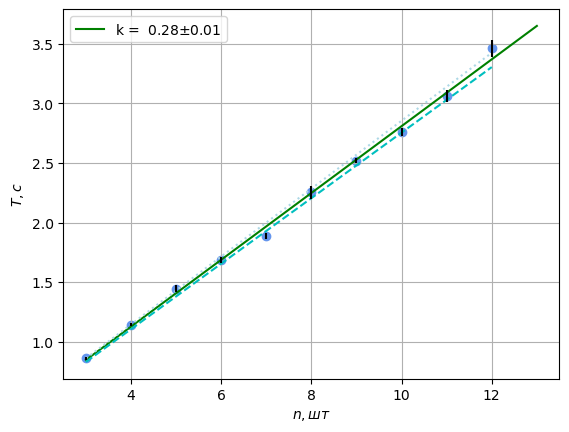
\includegraphics[width=12cm]{plot1.png}
    \caption{График зависимости периода колебаний от кол-ва магнитов $T(n)$}
\end{figure}

\begin{center}
    Из формулы 13 и графика находим $B_{\parallel} = (1.5 \pm 0.1)\cdot 10^{-5}$ Tл ($\varepsilon \approx 7.5\%$)
\end{center}
\newpage
\subsection*{Измерение вертикальной составляющей индукции магнитного поля Земли}
Для измерения $B_{\perp}$ будем уравновешивать момент, образованный вертикальной составляющей магнитного поля Земли, моментом сил грузиков, подвешенных к магнитной стрелке. Тогда условие равновесия:
\begin{equation}
    m_{\text{гр}}gr_{\text{гр}} = n\mathfrak{m}B_{\perp}
\end{equation}

\begin{table}[!h]
    \centering
    \begin{tabular}{|c|c|c|c|c|}
        \hline
        $n_{\text{ш}}$ & 10 & 8 & 6 & 4\\\hline
        $m_{\text{гр}}$, г&0.174 & 0.200 & 0.200 & 0.200\\\hline
        $r_{\text{гр}}$, см& 2.14 & 1.61 & 1.07 & 0.05\\\hline
        $M$, H$\cdot$ м $\cdot 10^{-5}$& $3.74 \pm 0.05$ & $3.22 \pm 0.04$ & $2.15 \pm 0.03$ & $1.07 \pm 0.01$\\\hline 
    \end{tabular}
    \caption{Зависимость момента сил тяжести груза от числа магнитов}
\end{table}

\begin{figure}[!h]
    \centering
    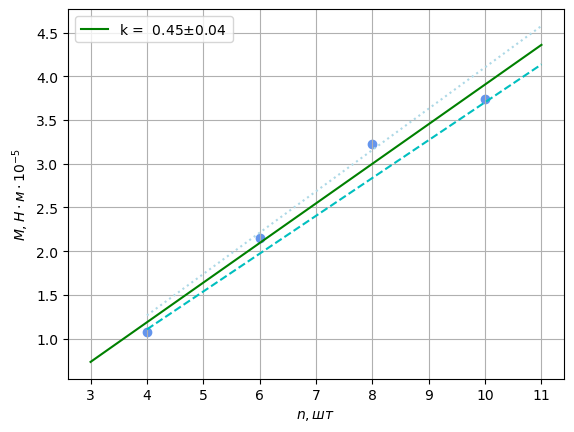
\includegraphics[width=12cm]{plot2.png}
\caption{Зависимость момента сил тяжести груза от числа магнитов $M_{\text{гр}}(n)$}
\end{figure}

\begin{center}
Из формулы (14) и гарфика получаем $B_{\perp} = (6.7\pm 0.8)\cdot 10^{-5}$ Tл ($\varepsilon\approx 12\%)$.
\end{center}
Теперь найдем магнитное наклонение $\beta:  \tg\beta = B_{\perp} / B_{\parallel} = 4.44 \pm 0.63 (\varepsilon\approx 14\%) \Rightarrow$ 
\begin{center}
$\beta = 77.3^{\circ} \pm 1.7^{\circ}; B = \sqrt{B_{\parallel}^2 + B_{\perp}^2} = (6.9 \pm 0.9)\cdot 10^{-5} \text{ Тл} (\varepsilon\approx 11.8\%)$
\end{center}

\indent
Оценим магнитный момент и магнитное отклонение магнитного поля Земли, считая ее однородно намагниченным шаром.
\begin{align}
    B_r = -\frac{\mu_0}{4\pi}\frac{3\mathfrak{m}\cos\varphi}{R^3} \hspace{1cm} 
    B_{\mathfrak{m}} = \frac{\mu_0}{4\pi}\frac{\mathfrak{m}}{R^3} \Rightarrow\\ 
    B_{\perp} = B_{\mathfrak{m}}\cos\varphi + B_r\hspace{1cm}
    B_{\parallel} = B_{\mathfrak{m}}\sin\varphi \Rightarrow\\ 
    tg\beta = 2\tg\varphi\hspace{1cm} \Rightarrow\hspace{1cm} \beta\approx 71^{\circ} (\varphi = 56^{\circ})
\end{align}

\subsection*{Выводы}
1)Вычислили магнитный момент неодимовых магнитов, сравив 2 способа его определения. 
$\mathfrak{m}_1 = 4.25\cdot 10^{-2}$ Дж/Тл и $\mathfrak{m}_1 = 6.70\cdot 10^{-2}$ Дж/Тл. Несмотря на то, что второй метод кажется менее точным, его относительная погрешность все равно оказалась меньше,чем первого метода.\\
2)C помощью магнитометра было измерено магнитная индукция у плюсов магнитного шарика $\approx 0.27$ Тл. Эта величина была также получена из формулы (8) при уже полученном магнитном моменте $\approx 0.68$ Тл. Видно, что занчения отличаются сильно и даже с учетом погрешности не совпадают. 
Так же была определена остаточная индукция $\approx 1.03$ Тл, что в пределах погрешности совпадает со справочными данными $1.1 - 1.4$ Тл.\\ 
3)С помощью крутильных колебаний магнитной "стрелки" была определена горизонтальная составляющая магнитного поля Земли $\approx 150$ мТл. Табличная величина для долгопрудного составляет $\approx 165$ мТл. Т.е полученный результат совпадает в пределах погрешности с табличной величиной.\\
4)Уравновешивая механический момент, действующий на магнитную "стрелку" мы определили значение вертикальной составляющей магнитного поля Земли $\approx 670$ мТл. Табличные данные для Долгопрудного $\approx 504$ мТл. В ворота погрешности это значение не попадает.\\
5)Мы также вычислили занчение магнитного отклонения $\approx 77^{\circ}$. Табличные данные для Долгопрудного $\approx 72^{\circ}$. В ворота погрешности так же не попадает.
